\documentclass{article}

% if you need to pass options to natbib, use, e.g.:
%     \PassOptionsToPackage{numbers, compress}{natbib}
% before loading neurips_2019

% ready for submission
% \usepackage{neurips_2019}

% to compile a preprint version, e.g., for submission to arXiv, add add the
% [preprint] option:
%     \usepackage[preprint]{neurips_2019}

% to compile a camera-ready version, add the [final] option, e.g.:
\usepackage[final]{neurips_2019}

% to avoid loading the natbib package, add option nonatbib:
%     \usepackage[nonatbib]{neurips_2019}

\usepackage[utf8]{inputenc} % allow utf-8 input
\usepackage[T1]{fontenc}    % use 8-bit T1 fonts
\usepackage{hyperref}       % hyperlinks
\usepackage{url}            % simple URL typesetting
\usepackage{booktabs}       % professional-quality tables
\usepackage{amsfonts}       % blackboard math symbols
\usepackage{nicefrac}       % compact symbols for 1/2, etc.
\usepackage{microtype}      % microtypography
\usepackage{graphicx}
\usepackage{float}


\newcommand{\vx}{\textbf{x}}
\newcommand{\vu}{\textbf{u}}
\newcommand{\ve}{\textbf{e}}
\newcommand{\fig}[2]{\includegraphics[width=#1\textwidth]{#2}}
\newcommand{\centerfig}[2]{\begin{center}\includegraphics[width=#1\textwidth]{#2}\end{center}}

\title{Improving Realism of Scene Graph to Image Generation}

\author{%
  Johann Lingohr \\
  \texttt{johannlingohr@gmail.com} \\
  \And
  Jiefei Li \\
  \texttt{jeffuvic@ece.ubc.ca} \\
  \And
  Jay Fu \\
  \texttt{ngaifu16@gmail.com} \\
}

\begin{document}

\maketitle

\section{Introduction}

Generating realistic images from text is one of the most interesting and challenging tasks in the field of artificial intelligence as it requires computer algorithms to precisely interpret human natural language and also have a sense of what ‘realism’ means in the visual world. With the rising popularity of the topic as well as recent developments in deep learning, there has been a significant focus on image generating algorithms. Generative adversarial networks (GANs) \cite{gan} have become one of the most standard neural network models used to generate realistic images. GANs have been shown to be extraordinarily powerful in generating realistic images and has been vastly leveraged in recent researches.

Although image generation with GANs seems promising, there has been many technical difficulties encountered in practice. In particular, generating realistic images from highly complicated sentences has remained unsolved as revealing the relational information between objects on the generated image is not a trivial task. We contribute to this problem by combining work generating images from text with work generating images from scene graphs. Specifically, we show that using scene graph embeddings to enforce relationship features and text embeddings to provide fine-grained image detail can help improve image generation. We first review existing work generating images from text and from scene graphs. We then provide an overview of our method. Afterwards we evaluate our model by performing experiments on the MS Coco Stuff dataset.

\section{Related Works}

Reed \textit{et al.} \cite{t2im} generate images using GANs conditioning on text and are able to generate high-resolution images. Huang \textit{et al.} \cite{stackedgan} further improve on this using a two-stage architecture resulting in 256x256 photo-realistic images. Xu \textit{et al.} \cite{attengan} go further by leveraging the attention mechanism to draw images region-by-region conditioned on relevant words in a long text description, resulting in images with much more detail. In a different approach Hong \textit{et al.} \cite{scenelayout} use text to predict the location of bounding boxes and infer the semantic layout of the image. Only after they predict a semantic layout do they generate images conditioned on the layout and a sentence embedding.
%This approach shows that we can break up hard tasks into manageable sub-tasks to improve results, going from coarse to fine level of detail in the process.
% Finally, Nvidia \cite{stylegan} incorporate style transfer to create a style-based image generator to replace the original generator in the GAN model, bringing the realism of synthesized images to an impressive level.

While these techniques generate realistic looking images when the input sentence describes simple scenes, they do not perform well when trying to generate images from complex scenes. One solution to this problem is to generate images conditioning on a scene graph in order to provide a systematic way to preserve object relationships in the image generation process. Johnson \textit{et al.} \cite{sg2im} use graph convolution neural networks (GCNs) to extract features and objects from scene graphs and are able to generate images that preserve relationships among multiple objects. However, their model does not incorporate attribute information and does not generate realistic images when there are multiple relationships among the objects. Tripathi \textit{et al.} \cite{sg2imgcontext} attempt to improve on this by introducing scene graph context to encourage generated images to appear realistic and better respect the scene graph relationships. However, they do not preserve scene graph attributes and do not clearly define scene graph context.

\section{Method}

\subsection{Graph Convolution Networks}

In order to generate images from scene graphs we first generate a scene layout similar to \cite{sg2im} and \cite{sg2imgcontext}. Given a scene graph $G = (V, E)$ where $V$ is the set of objects and $E$ is the set of relationship predicates $r_{ij}$ between a subject $s_i$ and an object $o_j$, a graph convolutional network computes a scene graph embedding by computing relationship embeddings and object embeddings. Given a triplet $(s_i, r_{ij}, o_j)$ we compute a relationship embedding \[\vx_{r_{ij}} = g_r(s_i, r_{ij}, o_j)\]where $g_r$ is a spatial graph convolution.

To compute object embeddings $\vx_{v_i}$ for an object $v_i \in V$, we consider all triplets in which $v_i$ appears as a subject and as an object: \[\vx_{v_i} = \sum_{s_i \in subj(v_i)} g_s(s_i, r_{ij}, o_i) + \sum_{o_i \in obj(v_i)} g_o(s_j, r_{ji}, o_i) \]where $subj(v_i)$ is the set of nodes in which object $v_i$ acts as subject, $obj(v_i)$ is the set of nodes in which object $v_i$ acts as object, and $g_s$ and $g_o$ are spatial graph convolutions.

Processing scene graphs with graph convolution networks produces embedding vectors $\vx_{v_i}$ that aggregate information across objects and relationships in the graph. \cite{sg2im} use an object embedding $\vx_{v_i}$ to predict a bounding box $\hat{b}_i = (x_0, y_0, x_1, y_1)$ and a binary mask $\hat{m}_i$ for each object, from they generate a scene layout by warping the masks to the bounding boxes. The scene layout is then concatenated with random noise and used as input into a cascading refinement network to generate the images.

\subsubsection{Scene Graph Context}

\cite{sg2imgcontext} introduce a scene context network to pool context features in the graph convolution network that are used to produce context embeddings. These embeddings are used in the image generator to encourage images to respect scene graph relationships by conditioning image generation on context embeddings. We believe, however, that conditioning image generation on context in this manner is incorrect due to scene graph sparsity, a problem in which scene graph relationships between objects are not fully specified and even contain disconnected components. Since scene layout is finalized at this point, using context embeddings after scene layout is generated does not effectively improve spatial relationships.

We instead propose using global scene graph context to condition bounding box predictions. Specifically, we compute a global context vector $\vu$ by \[ \vu = \frac{1}{|E|}\sum_{\ve \in E} \ve .\]We then predict bounding boxes conditioned on global context by \[\hat{b}_i = g_b(v_i | \vu) \]where $g_b$ is the bounding box prediction network. We hypothesize this will better encourage generated images to respect scene graph relationships, especially in scene graphs with few connections and disconnected components.

However, this only conditions the coordinates of bounding boxes on global context. We also use global context to generate segmentation masks by \[ \hat{m}_i = g_m(v_i | \vu) \]where $g_m$ is the mask regression network. We hypothesize conditioning segmentation masks on global context will improve image realism and diversity.

\subsection{Embedding Captions}
\begin{figure}[H]
    \centering
    \includegraphics[width=\textwidth]{532Pres.jpeg}
    \caption{The caption input is processed by a pre-trained LSTM network, whose last hidden unit is passed to a fully connected network to generate caption embedding.}
    \label{fig:Model}
\end{figure}
A limitation of previous work generating images from scene graphs is that they remove all attribute information such as size and colour from scene graphs and as a consequence limit model capacity. This problem is further exacerbated by scene graph sparsity and so generating images using only scene graphs does not generate realistic looking images. For example, if most of the trees in the training dataset are in green color, the model can only guess the generated tree would also be in green even if the input sentence contains the key word “red tree” explicitly. To overcome this problem we also take image captions as the second input of the model and produce caption embeddings containing attribute information from the original sentence (see Figure 1). Specifically, for each image we process a corresponding caption using a 2-layer LSTM to produce a final hidden state with 650 units. We then concatenate the hidden state with random noise and create a caption embedding by feeding the vector into a fully connected network. The resulting embedding has dimension 128 and is spatially replicated to the dimensions of the scene layout before being passed into a series of upsampling layers.

% For simplicity, we used a pre-trained 2-layer LSTM model to process the caption inputs. The last hidden cell unit is used as it embeds all the information in the sentence. Note that due to the limited GPU memory, we only use the cell from the second LSTM layer. The cell unit has dimension 650. A noise vector of size 128 is then concatenated with the cell to introduce randomness to the model. The resulted vector is fed into a fully connected network which map the caption embedding to dimensions of $128 \times 64 \times 64$ where 128 is the number of channel and $64 \times 64$ matches the dimension of scene layout. The caption embedding is finally concatenated with scene layout to be passed into a series of upsampling layers.

\subsection{Loss}

As a baseline we follow \cite{sg2im} and \cite{sg2imgcontext} by training an image generator $G_{img}$ conditioned on inputs, scene layout, and scene context embedding, jointly with an image discriminator $D_{img}$ and object discriminator $D_{obj}$. The network is trained to minimize the weighted sum of six losses:
\begin{itemize}
\item \textit{Box Loss} $L_{box}$ penalizing the $L_1$ difference between coordinates of the ground-truth bounding box and predicted bounding box
\item \textit{Mask Loss} $L_{mask}$ penalizing differences between ground truth masks and predicted masks
\item \textit{Pixel loss} $L_{pix}$ penalizing the $L_1$ pixel-wise difference between ground-truth image and generated image
\item \textit{Adversarial image loss} $L_{GAN}^{img}$ from $D_{img}$ that encourages generated images to be realistic and relevant to the scene context
\item \textit{Adversarial object loss} $L_{GAN}^{obj}$ from $D_{obj}$ that encourages objects to appear realistic
\item \textit{Auxiliary classifier loss} $L_{AC}^{obj}$ from $D_{obj}$ encouraging generated objects to be classified by the object discriminator
\end{itemize}
\subsection{Training}
We train our model using Adam \cite{adam} with a learning rate $10^{-4}$ and batch size 16 for 330 thousand iterations. We note that we intended to train the final model on 1 million iterations, following Johnson \textit{et al.}, but the extra model parameters required halving our expected batch size from 32 to 16 and so could only train 5 days on a single Gtx 2080Ti.

\section{Experiments}
In order to evaluate a generated image we need a measure that answers 1) how realistic does the generated image appear? 2) how well can we recognize the different objects in the image? 3) How diverse are the generated images? To this end we use the Inception Score \cite{inception}\cite{inceptionscorer}, which evaluates both the quality of generated images and diversity by applying a pre-trained classifier on generated images. Correctly predicting class labels for objects in the generated image should correspond to the generated images looking realistic. We also used Intersection-over-union score to evaluate the quality of our predicted bounding boxes.

\subsection{Dataset}
We train our model to generate $64 \times 64$ images on the COCO-Stuff \cite{cocostuff} dataset. The COCO-Stuff dataset contains 40k training and 5k validation annotated images with bounding boxes and segmentation masks, as well as providing 80 thing categories and 90 stuff categories. Similar to \cite{sg2im} and \cite{sg2imgcontext}, the segmentation masks and the bounding boxes labelled in COCO stuff can be used as ground truth to train the Graph Convolution Network to predict desired scene layout. We can also use the image captions and annotations in COCO to construct scene graphs based on the 2D image coordinates of the objects. These scene graphs specify six geometric relationships: \textit{left of}, \textit{right of}, \textit{above}, \textit{below}, \textit{inside}, and \textit{surrounding}. We pass the scene graphs to the image generator to create scene layout and then synthesize photographic images. Images that have too few or too many objects are filtered out, which leaves 24,972 train images and 1024 validation and 2050 test images.

\subsection{Qualitative Results}
Figure \ref{fig:example context} compares examples generated by Johnson \textit{el al.} and our model. We conclude that although our model is able to produce images respecting spatial relationships, our results are blurrier and the objects less recognizable. The bottom row of Figure \ref{fig:example context} shows the predicted scene layout. We see although our model is able to correctly localize bounding boxes, for example, the location of the tie on the man, we do not always produce reasonable bounding box shapes, for example, that skateboards are rectangular and not square.
\begin{figure}[]
    \centering
    \includegraphics[width=\textwidth]{Figure5.png}
    \caption{Samples generated using a group of example scene graphs provided by the baseline model. For each sample, we show its scene graph, caption, baseline image, our image, our image without using caption and layout prediction.}
    \label{fig:example context}
\end{figure}

\subsection{Quantitative Results}

\textbf{Inception Score}. We evaluate the quality and diversity of generated images by computing the inception scores on a set of manually generated scene graphs. We also compute this score for the baseline model and summarize results in table \ref{Example Context}. We observe that our inception score does not beat the baseline model, but reaches about 78\% of the baseline score using significantly fewer iterations. We also generate images without using captions (feeding pure random noise as caption embedding) and observe minor difference in inception score. While only minor differences, this suggests for a fully-trained model that adding sentence captions can add detail to generated images and improve realism.
\begin{table}[H]
    \centering
    \begin{tabular}{|l|l|}
    \hline
    Method               & Inception \\ \hline
    Ours(Full Model)     & 2.71     \\
    Ours(Use no caption) & 2.60      \\ \hline
    Baseline(Full Model) & 3.46       \\ \hline
    \end{tabular}
    \caption{Inception scores for images generated from example scene graphs provided by Johnson \textit{et al.} \cite{sg2im}. We provide the scores for the baseline model for comparison.}
    \label{Example Context}
\end{table}

\textbf{IOU Score}. We evaluate how well our model generates images that respect geometric relationships using intersection over union (IOU) of bounding boxes. The IOU score evaluates the quality of a scene layout by calculating the intersection between ground truth layout and the predicted layout. From Table \ref{IOU} we see we achieve an average IOU of 0.496 on the test set, which slightly outperforms the baseline model.
\begin{table}[H]
    \centering
    \begin{tabular}{|l|l|l|}
    \hline
    Metric      & Baseline & Ours           \\ \hline
    Average IOU & 0.462    & \textbf{0.496} \\ \hline
    \end{tabular}
    \caption{Intersection Over Union score on  COCO Stuff test set}
    \label{IOU}
\end{table}
\subsection{Ablation Study}
We also conduct an ablation study to evaluate the the importance of each component of our model. Considering our study scale, we perform this study in a way that avoids retraining models.
 \begin{itemize}
   \item \textbf{No predicted layout}. Use ground truth bounding boxes and segmentation masks to create scene layout.
   \item \textbf{No predicted bounding box}. Create scene layout using GT bounding boxes and predicted segmentation.
   \item \textbf{No predicted segmentation mask}. Create scene layout using GT segmentation asks and predicted bounding boxes.
   \item \textbf{No image caption}. Concatenate pure random noise with the scene layout instead of caption embedding when generating input to CRN.
 \end{itemize}
For each case we generate 5 images and average the inceptions score over all generated images in the same sampling iteration. We also generate images using the baseline model for comparison and summarize results in Table \ref{Ablation Study}.
\begin{table}[H]
    \centering
    \begin{tabular}{|l|l|}
    \hline
    Method                & Inception          \\ \hline
    Ours(Full Model)      & $3.97 \pm 0.04$          \\
    Ours(GT Layout)       & \textbf{$6.78\pm0.01$} \\
    Ours(Bbox GT)         & $3.98\pm0.02$          \\
    Ours(Mask GT)         & $5.28\pm0.01$          \\
    Ours(Without Caption) & $3.41\pm0.1 $          \\ \hline
    Baseline(Full Model)  & $5.63\pm0.1 $          \\
    Baseline(GT Layout)   & $5.73\pm0.1$           \\ \hline
    \end{tabular}
    \caption{Ablation study using Inception Scores. We sampled the test sets for 5 times and report the mean and standard deviation across five attempts. The baseline model was tested on the same test set for five times and the average inception scores are also provided as comparisons.}
    \label{Ablation Study}
\end{table}
We observe our full model produces a lower score compared to the baseline (3.97 vs 5.63). However, using ground truth scene layout our models performs better than baseline (6.78 vs 5.73). When only using the ground truth segmentation masks the inception score drops by 22\% (6.78 vs 5.28) and when only using ground truth bounding boxes drops significantly lower (6.78 vs 3.98). This result indicates that the our predicted bounding box is comparable with the ground truth bounding box which confirm the previous IOU result. However, the quality of our predicted segmentation is still poor compared with ground truth. Finally, without using sentence captions the score drops by 14\% compared with the full model score (3.41 vs 3.97), which shows the positive effect of caption embedding.

We further qualitatively compare our model with Johnson \textit{et al.}'s by generating images for 7 randomly selected test images, which can be seen in Figure \ref{fig:Ablation}. It appears our full model performs worse than baseline using predicted scene layout, but produces better results when using ground truth scene layout. This is very likely a result of not training the model long enough. We also observe worse results when not using caption embeddings. This suggests that caption embeddings are important to the generation of more fine-grained details.

\begin{figure}
    \centering
    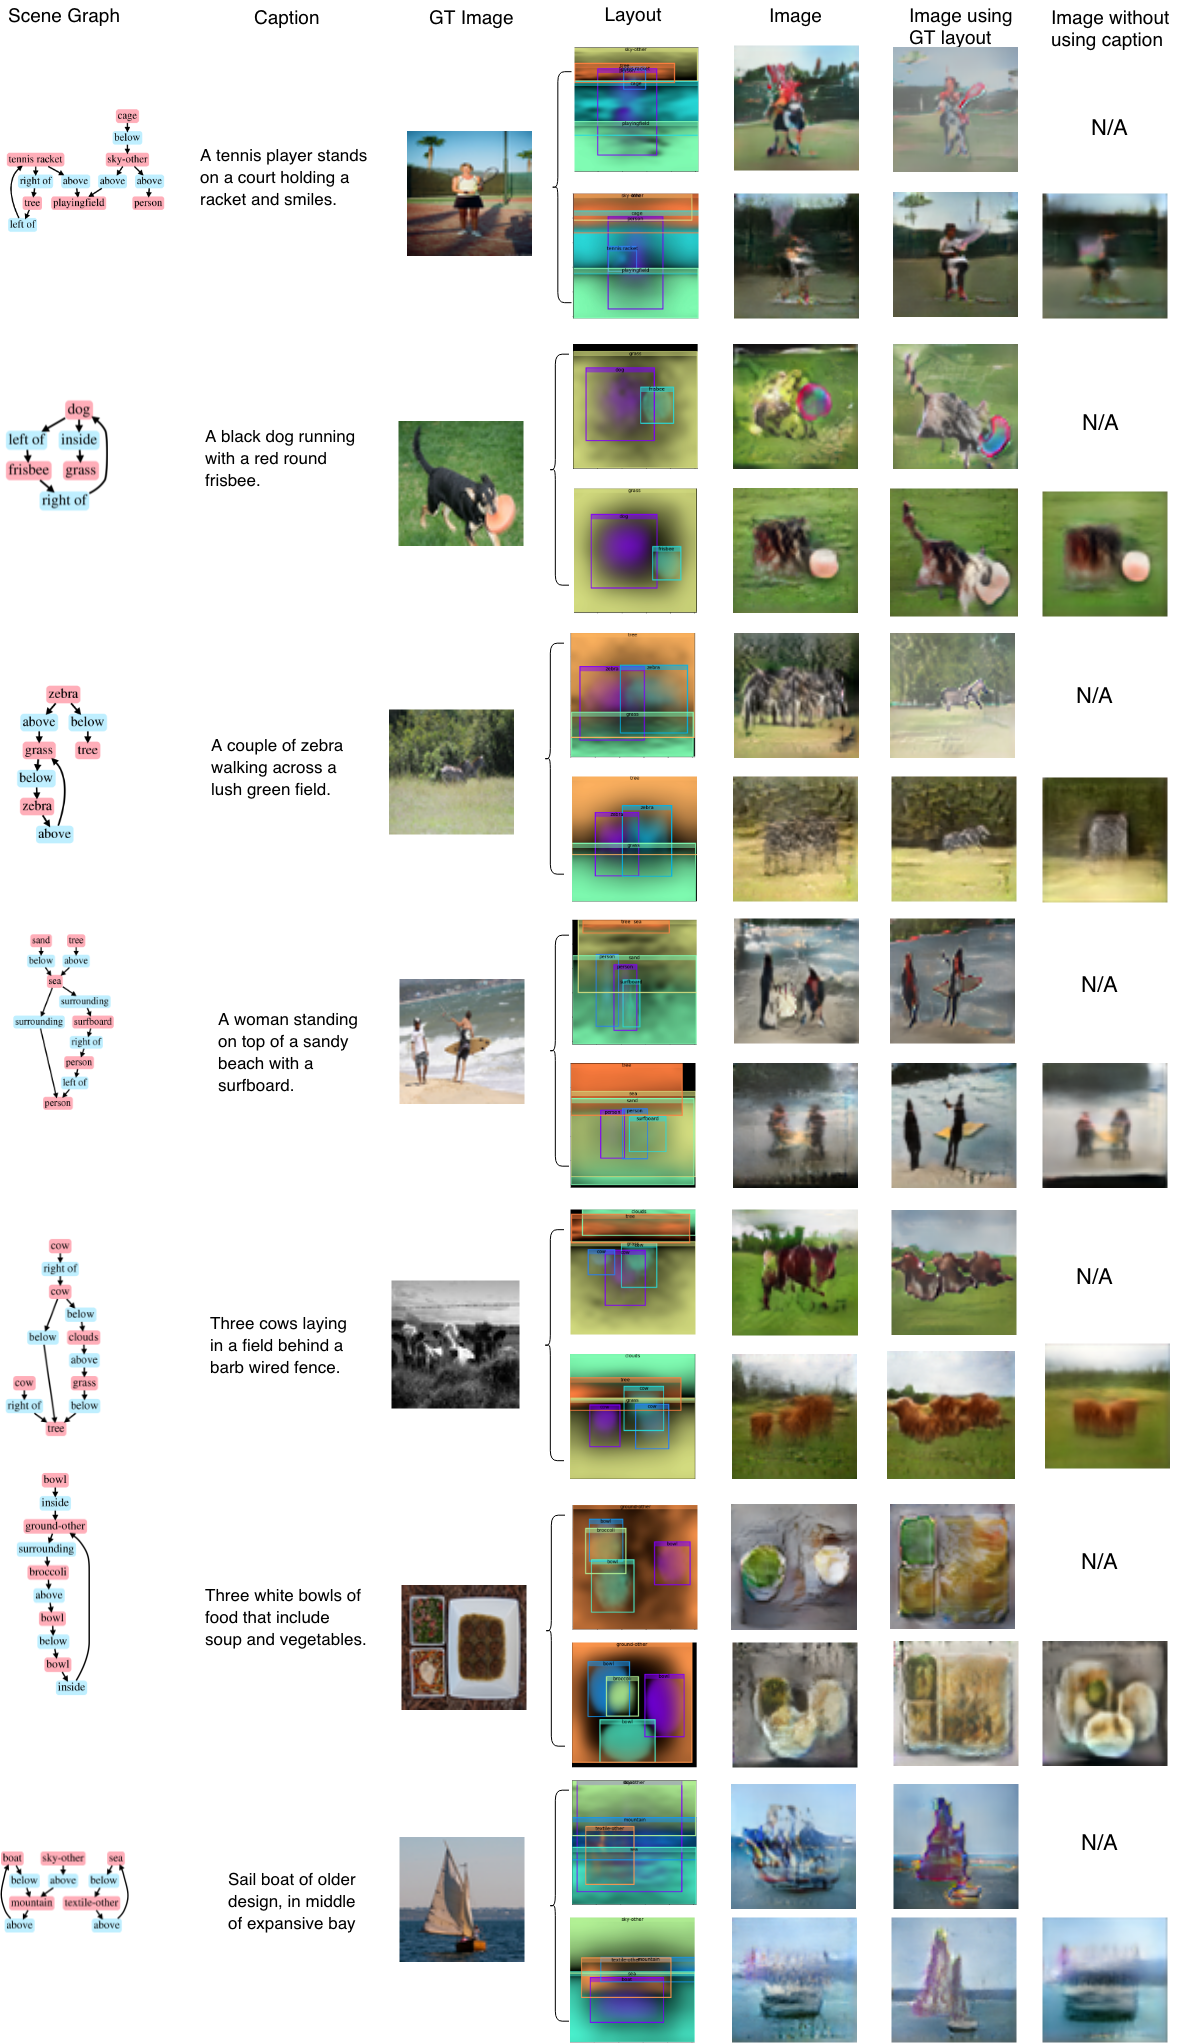
\includegraphics[height=\textheight]{7_samples.png}
    \caption{For each COCO test sample, we show its scene graph, caption, layout prediction, image generation, image generation without using caption, image generation using GT layout. We also provide score for the baseline model for comparison. For each pair of rows, the first row shows the baseline results and the second row shows our results.}
    \label{fig:Ablation}
\end{figure}
\subsection{Discussion}
Qualitatively we observe our models performs better in Figure \ref{fig:Ablation} than in Figure \ref{fig:example context}. One possible reason is that the scene graphs are generated dynamically and so are not deterministic. This means the quality of scene graphs can vary and so it is possible the scene graph quality varies between figures. Another possible reason could be that the captions in Figure \ref{fig:example context} are synthesized from corresponding scene graphs, which is less meaningful semantically because they do not introduce any new semantic information, but present the same information in a different way. We would expect, therefore, that using proper captions would introduce more meaningful information and which have a positive impact on output quality.

\section{Future Work}
Due to the limited time and hardware resources we used a pre-trained LSTM model. However, the performance could be improved by fine-tuning the model and perhaps exploring other sentence embedding models with different structures such as a bi-directional LSTM or GRU. Another line of work could explore different ways in which to include caption embeddings into the model, for example, by also conditioning scene layout on text similar to Hong \textit{et al.} \cite{scenelayout}.

Further work can also improve the discriminator since our work primarily focuses on improving the generator and we do not mirror all changes in the discriminator. We can correspondingly modify the discriminator to balance our changes and improve overall training. Informed by \cite{inceptionscorer} and \cite{sg2imgcontext}, both IOU and inception score are not the best evaluation methods for GAN and scene layout, a better evaluation metric should be explored, and user study should be added into the study.

Finally, future work can look further into scene graph embeddings. Due to the sparsity and even disconnected nature of some scene graphs it might be possible to improve relationships between objects in scene graphs if we could find a better way infer relationships between objects separated in a graph. This should help image generation by enforcing more cohesion between objects in the scene graph.

\section{Conclusion}
In this paper we address the problem of generating images from scene graphs, extending Johnson \textit{et al.}'s model by incorporating global relational context to condition bounding box and segmentation mask predictions. We also borrow from text-to-image methods and enhance our model by conditioning the coarse-to-fine image generator on textual caption embeddings. Although we present an incompletely trained model, using only 330k iterations instead of the intended 1 million, our preliminary results suggest our method has the potential to improve conditional image generation. Further work can try to validate our results by also training on the Visual Genome dataset.

\bibliographystyle{unsrt}
\begin{thebibliography}{1}

\medskip
\small

\bibitem{gan}
Ian J. Goodfellow,
Jean Pouget-Abadie, Mehdi Mirza, Bing Xu, David Warde-Farley, Sherjil Ozair,Aaron Courville and Yoshua Bengio.
\newblock Generative Adversarial Nets, 2014;
\newblock arXiv:1406.2661.

\bibitem{t2im}
Scott Reed, Zeynep Akata, Xinchen Yan, Lajanugen Logeswaran, Bernt Schiele and Honglak Lee.
\newblock Generative Adversarial Text to Image Synthesis, 2016;
\newblock arXiv:1605.05396.

\bibitem{stackedgan}
Xun Huang, Yixuan Li, Omid Poursaeed, John Hopcroft and Serge Belongie.
\newblock Stacked Generative Adversarial Networks, 2016;
\newblock arXiv:1612.04357.

\bibitem{attengan}
Tao Xu, Pengchuan Zhang, Qiuyuan Huang,
Han Zhang, Zhe Gan, Xiaolei Huang and Xiaodong He.
\newblock AttnGAN: Fine-Grained Text to Image Generation with Attentional Generative Adversarial Networks;
\newblock arXiv:1711.10485.


\bibitem{sg2im}
Justin Johnson, Agrim Gupta and Li Fei-Fei.
\newblock Image Generation from Scene Graphs, 2018;
\newblock arXiv:1804.01622.

\bibitem{sg2imgcontext}
Subarna Tripathi, Anahita Bhiwandiwalla, Alexei Bastidas and Hanlin Tang.
\newblock Using Scene Graph Context to Improve Image Generation, 2019;
\newblock arXiv:1901.03762.

\bibitem{scenelayout}
Seunghoon Hong, Dingdong Yang, Jongwook Choi and Honglak Lee.
\newblock Inferring Semantic Layout for Hierarchical Text-to-Image Synthesis, 2018;
\newblock arXiv:1801.05091.

\bibitem{adam}
Diederik P. Kingma and Jimmy Ba.
\newblock Adam: A Method for Stochastic Optimization, 2014;
\newblock arXiv:1412.6980.

\bibitem{inception}
Tim Salimans, Ian Goodfellow, Wojciech Zaremba, Vicki Cheung, Alec Radford and Xi Chen.
\newblock Improved Techniques for Training GANs, 2016;
\newblock arXiv:1606.03498.

\bibitem{inceptionscorer}
Shane Barratt and Eishi Sharma.
\newblock A Note on the Inception Score, 2018;
\newblock arXiv:2018.01973.

\bibitem{cocostuff}
Holger Caesar, Jasper Uijlings and Vittorio Ferrari.
\newblock COCO-Stuff: Thing and Stuff Classes in Context, 2016;
\newblock arXiv:1612.03716.


\end{thebibliography}

\end{document}
